%!TEX root=../../../main.tex

Exporting metadata in a syntactically standard format is a necessary step
towards interoperability between systems collecting user annotations, but not a
sufficient one. The semantics of metadata also need to have an agreed form;
in the context of RDF, applications exporting annotations could also supply an
ontology which describes what the meaning of data is.

The Open Annotation \cite{ref:oa} data model (denoted by \textit{OA} in the
rest of this document) is a specification proposed by W3C that aims at solving
this exact issue. It proposes a general vocabulary of terms that can be used to
describe the most common use-cases of annotations.

The minimal basis of OA is defined as an RDF graph in which annotations have a
target identified by an IRI, and a body; an example graph is included in
Figure \ref{fig:oa}. Further restrictions regarding the types of these elements
are not enforced; for example, the target of an annotation can be another
annotation. Nevertheless, it is expected that the type is specified when
serialising the representation, in order to facilitate third-party consumption.

\begin{figure}[!ht]
  \centering
  \fbox{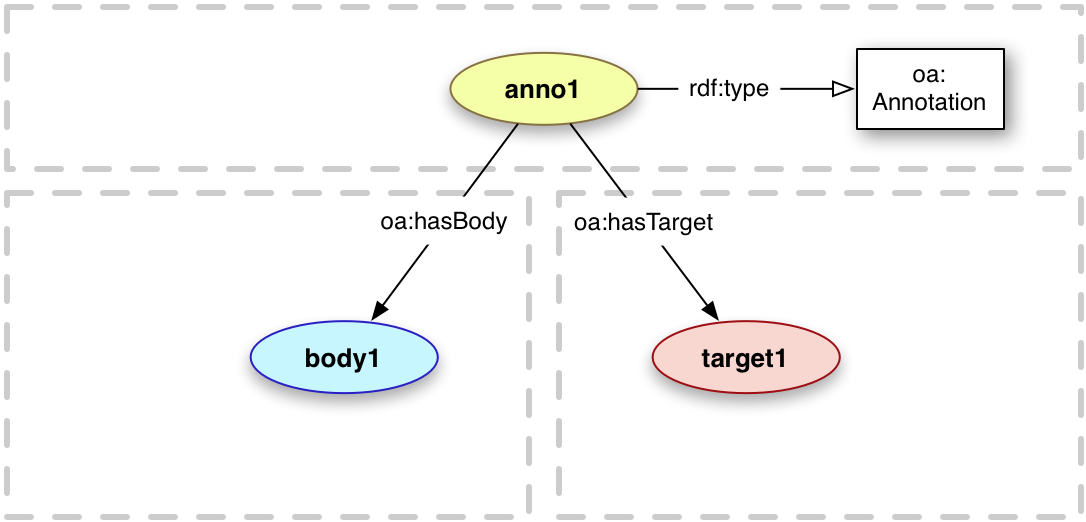
\includegraphics[scale=0.7]{static/img/oa.png}}
  \caption[Basic Open Annotation RDF Graph]
          {Basic Open Annotation RDF Graph, source \cite{ref:oa}. Annotations
           need to specify a body and target identified by an IRI (e.g., a
           Web page).}
  \label{fig:oa}
\end{figure}

\newpage

The body and target attributes can be extended by adding miscellaneous attributes.
For example, Figure \ref{fig:oahubble} presents an annotation where the target
is constrained to a specific region of an image. Similarly, the body can also
be constrained; for instance, it could be specified that only certain pages of
a textbook are describing a target image.

\begin{figure}[!ht]
  \centering
  \fbox{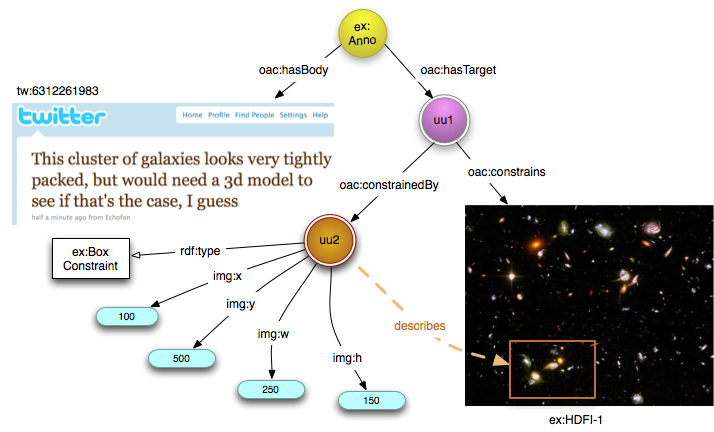
\includegraphics[scale=0.64]{static/img/oahubble.png}}
  \caption[Twitter message used to annotate an image region using Open Annotation.]
          {More complex example usage of Open Annotation, source \cite{ref:oahubble}.
           A Twitter message is used as the body for an annotation targeted at a
           specific region of an image. The \textit{target} attribute points at the whole
           image IRI, but is constrained by rectangle coordinates
           ($x, y, w, h$).}
  \label{fig:oahubble}
\end{figure}

Other elements supported by OA include annotation tagging, versioning the
target or body or constraints on the validity of the annotation (e.g., HTTP
headers than need to be used to retrieve the correct target). Further details
can be found in the specification \cite{ref:oa}.

As Open Annotation model instances are RDF graphs they can be exported in any
of the supported serialisation formats; the guideline is to use JSON-LD
\cite{ref:oa}, the option being further explored by this project, with details
in Section \ref{sec:diss}.
